\documentclass[10pt]{beamer}

\usetheme[progressbar=foot]{metropolis}
\usepackage{appendixnumberbeamer}

\usepackage{booktabs}
\usepackage[scale=2]{ccicons}

\usepackage{pgfplots}
\usepgfplotslibrary{dateplot}

\usepackage{xspace}
\usepackage{xcolor}

\DeclareMathOperator{\stdev}{stdev}
\DeclareMathOperator{\var}{var}
\DeclareMathOperator{\cov}{cov}
\DeclareMathOperator{\corr}{corr}
\DeclareMathOperator{\prob}{prob}
\DeclareMathOperator{\n}{n}
\DeclareMathOperator{\N}{N}
\DeclareMathOperator{\Cov}{Cov}

\newcommand{\hlf}{\frac{1}{2}}
\newcommand{\bi}{\begin{itemize}}
\newcommand{\ei}{\end{itemize}}
\newcommand{\im}{\item}
\newcommand{\D}{\mathrm{d}}
\newcommand{\E}{\mathrm{e}}
\newcommand{\mye}{\ensuremath{\mathsf{E}}}
\newcommand{\myreal}{\ensuremath{\mathbb{R}}}
\newcommand{\bq}{\begin{equation}}
\newcommand{\eq}{\end{equation}}
\newcommand{\eqdef}{\;\buildrel \text{d{}ef}\over = \;}
\newcommand{\xstar}{\buildrel *\over X}
\newcommand{\pmax}{p^{\text{max}}}
\newcommand{\qmax}{q^{\text{max}}}
\newcommand{\bfr}{\begin{frame}}
\newcommand{\bfrp}{\begin{frame}[plain]}
\newcommand{\efr}{\end{frame}}
\newcommand{\F}{\mathcal{F}}
\newcommand{\FF}{\mathbb{F}}
\newcommand{\ve}{\varepsilon}
\newcommand{\lh}{\hat{\lambda}}
\definecolor{mycolor}{gray}{0.8}
\definecolor{mymaincolor}{rgb}{0.6862745098039216,0.9333333333333333,0.9333333333333333}
\newcommand{\alr}[1]{\textcolor{blue}{#1}}
\definecolor{LightCyan}{rgb}{0.88,1,1}
\newcommand{\yel}{\cellcolor{yellow}}
\newcommand{\blue}{\cellcolor{SkyBlue}}
\newcommand{\gr}{\cellcolor{SpringGreen}}
\newcommand{\pink}{\cellcolor{pink}}
\newcommand{\apr}{\cellcolor{Apricot}}
\newcommand{\tve}{\tilde{\varepsilon}}
\newcommand{\tw}{\tilde{w}}
\newcommand{\ttth}{\tilde{\theta}}
\newcommand{\te}{\tilde{e}}
\newcommand{\ts}{\tilde{s}}
\newcommand{\tx}{\tilde{x}}
\newcommand{\ty}{\tilde{y}}
\newcommand{\tv}{\tilde{v}}
\newcommand{\tp}{\tilde{p}}
\newcommand{\tF}{\tilde{F}}
\newcommand{\tf}{\tilde{f}}
\newcommand{\tZ}{\tilde{Z}}
\newcommand{\ow}{\overline{w}}
\newcommand{\lb}{\left[}
\newcommand{\rb}{\right]}
\newcommand{\lp}{\left(}
\newcommand{\rp}{\right)}
\newcommand{\tm}{\tilde{m}}
\newcommand{\tc}{\tilde{c}}
\newcommand{\tz}{\tilde{z}}
\newcommand{\str}[1]{\textcolor{blue}{\sout{#1}}}
\newcommand{\tr}{\widetilde{R}}
\newcommand{\tR}{\widetilde{\mathbf{R}}}
\newcommand{\bms}{\begin{multline*}}
\newcommand{\ems}{\end{multline*}}
\newcommand{\bas}{\begin{align*}}
\newcommand{\eas}{\end{align*}}
\newcommand{\qr}{\mathbb{Q}}
\newcommand{\IMAGES}{/home/kerry/Dropbox/Images}
\newcommand{\tX}{\tilde{X}}
\newcommand{\tY}{\tilde{Y}}

\setbeamertemplate{frame footer}{Chapter 1, BUSI 521, Spring 2024}

\title{Chapter 1: Utility and Risk Aversion}

\date{}
\author{Kerry Back\\ 
BUSI 521/ECON 505\\
Spring 2024\\
Rice University}


\begin{document}

\maketitle

\begin{frame}{Outline}
  \bi 
  \im Quick overview of finance
  \im Utility functions and risk aversion coefficients
  \im Certainty equivalents
  \ei
\end{frame}

\section{Overview of Finance}


\begin{frame}{Examples of Finance Questions}

\begin{enumerate}
\item A company can invest $K$ to generate an uncertain cash flow of $\tilde{x}$ in one year.  Should it make the investment?
\item If the company needs to raise the capital, under what conditions will it choose debt versus equity financing?
\item What is the optimal portfolio of stocks for an investor?
\item Which of two stocks should have the higher expected return?
\item What is the most efficient way to organize the buying and selling of stocks?
\end{enumerate}
\end{frame}

\section{Utility Functions}

\begin{frame}{Utility and Risk Aversion}
\bi

\im Expected utility $\mye[u(\tilde{w})]$
\bi
\im Utility function $u$ is unique up to monotone affine transform: $f(w) = a+b u(w)$ for $b>0$.
\ei

\im Risk aversion: $\mye[\tilde{\varepsilon}]=0 \Rightarrow \mye[u(w+\tilde{\varepsilon})] < \mye[u(w)]$.
\bi
\im Equivalent to concavity (Jensen's inequality)
\im Equivalent to decreasing marginal utility: $u'' \leq 0$.
\im Invariant under monotone affine transformations.
\ei

\ei
\end{frame}




\begin{frame}{Coefficients of Risk Aversion}
\bi    
\im Absolute risk aversion: $\alpha(w) = -u''(w)/u'(w)$
\im Risk tolerance: $\tau(w) =  1/\alpha(w)$
\im Relative risk aversion: $\rho(w) = w\alpha(w) = - wu''(w)/u'(w)$.
\ei
\end{frame}


\begin{frame}{Some Special Utility Functions}
\bi
    
\im CARA = Constant Absolute Risk Aversion
\bi 
\im $u(w) = - \E^{-\alpha w}$
\im $\alpha$ is the coefficient of absolute risk aversion.
\ei 

\im CRRA = Constant Relative Risk Aversion 
\bi
\im 
$u(w) = \log w \Rightarrow$ relative risk aversion $ = 1$
\im $u(w) = w^{1-\rho}/ (1-\rho) \Rightarrow$ relative risk aversion $=\rho$
\ei

\ei
\end{frame}

\begin{frame}{CRRA Utility Functions}
  \begin{center}
  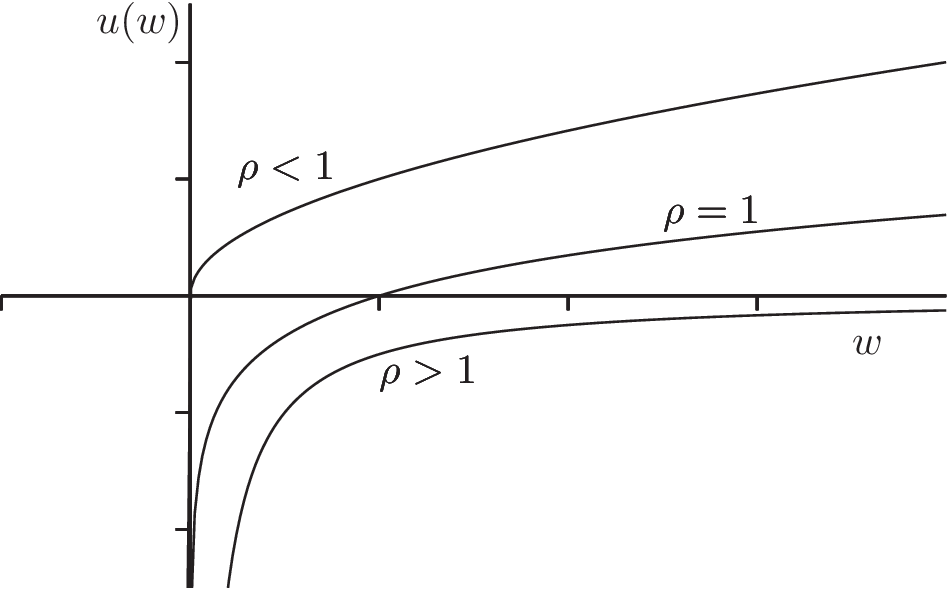
\includegraphics{images/fig1_4.png}
  \end{center}
  \end{frame}

\begin{frame}{Proof that CARA = $-\E^{-\alpha w}$}
 The coefficient of absolute risk aversion is
 $$-\frac{u''(w)}{u'(w)} = - \frac{\D \log u'(w)}{\D w}$$
 CARA means this is constant.  Call it $\alpha$. Then $\log u'$
 is an affine (constant plus linear) function of $w$ with slope $-\alpha$.  This means
\begin{align*}
    \log u'(w) = \log u'(0) - \alpha w &\Rightarrow u'(w) = u'(0)\E^{-\alpha w}\\
& \Rightarrow u(w) = u(0) + u'(0)\int_0^w \E^{-\alpha x}\,\D x\\
& \Rightarrow u(w) = u(0) - \frac{u'(0)}{\alpha} \left(\E^{-\alpha w} - 1\right)
\end{align*}
\end{frame}

\begin{frame}{Linear Risk Tolerance}
  \bi
  \im CARA risk tolerance $\,= 1/\alpha$
  \im CRRA absolute risk aversion $\,= \rho/w$.  Risk tolerance $\,= w/\rho$
  \im Linear risk tolerance: $\tau(w) = A + B w$.
  \bi
  \im For CARA, $A=1/\alpha$, $B=0$
  \im For CRRA, $A=0$, $B = 1/\rho$
  \im In general, $B$ is called the cautiousness parameter.
  \ei
  \ei
  \end{frame}
  
  \begin{frame}{LRT Utility Functions with $B>0$}
  \bi
  \im CARA
  \im CRRA
  \im Shifted CRRA
  \bi
  \im Shifted log: $u(w) = \log (w-\zeta)$
  \im Shifted power: $u(w) = \frac{1}{1-\rho}(w-\zeta)^{1-\rho}$
  \ei
  \ei
  \end{frame}
  
  \begin{frame}{Quadratic Utility}
   $$u(w) = -\frac{1 }{2}\left(\zeta-w\right)^2$$ 
  \bi
  \im Quadratic utility is monotone increasing for $w<\zeta$ ($\zeta$ is bliss point).
  \im Risk tolerance: $\tau(w) = \zeta-w$, so $A=\zeta$ and $B=-1$.   
  \im Implies mean-variance preferences:
  $$\mye[u(\tilde{w})] \;\;\sim  \;\;\zeta \overline{w} - \frac{1}{2}\overline{w}^2 - \frac{1}{2}\var(\widetilde{w})$$
  \ei
  \end{frame}
  
  \begin{frame}{Decreasing Absolute Risk Aversion}
    \bi
    \im An investor has DARA utility if absolute risk aversion $\alpha(w)$ is a decreasing function of $w$.
    \im CRRA utility is DARA: $\alpha(w) = \rho/w$ for a constant $\rho$ (relative risk aversion).
    \im LRT utility with $B>0$ is DARA.
    \im Quadratic utility is not DARA.
    \ei
    end{frame}


\section{Certainty Equivalents}

\begin{frame}{Certainty Equivalents}
  \bi
  \im A constant $x$ is the certainty equivalent of a random $\tilde{w}$ if $u(x) = \mye[u(\tilde{w})]$.  
\im Risk aversion implies $x<\mye[\tilde{w}]$.
\im Certainty equivalents are invariant under monotone affine transformations.
\ei
\end{frame}

\begin{frame}{CARA Utility and Normal Gambles}
  \bi
  \im CARA investor with a normally distributed wealth having mean $w$. How much less than $w$ is the certainty equivalent?
  \im Equivalent question: CARA investor with initial wealth $w$ facing a \alert{zero-mean} normally distributed gamble.  How much would she pay to avoid the gamble?
  \im Answer: would pay $\alpha \sigma^2/2$ where $\sigma^2$ is the variance of the gamble.
  \im Higher risk aversion $\Rightarrow$ pay more.  Higher risk $\Rightarrow$ pay more.
  \ei
\end{frame}

\begin{frame}{Proof}
  \bi
   \im Call the gamble $w + \sigma \tve$ where $\tve$ is a standard normal.
   \im Call the certainty equivalent $x$.  Define $\pi = w-x$, so the certainty equivalent is $w-\pi$.
   \im Claim is that $\pi = \alpha\sigma^2/2$.
   \pause
   \im The definition of the certainty equivalent and negative exponential (CARA) utility tell us that $\pi$ satisfies
  \begin{align*}
  u(w-\pi) &= \mye\left[u(w+\sigma\tilde{\varepsilon})\right] \\
   \Leftrightarrow \qquad -\E^{-\alpha(w-\pi)} &= \mye\left[-\E^{-\alpha(w+\sigma\tilde{\varepsilon})}\right]
  \end{align*} 
  \ei
\end{frame} 

\begin{frame}[plain]
  \bi
  \im Use the following fact: if $\tilde{x}$ is normal $(\mu,\sigma)$, then 
  $$\mye\left[\E^{\tilde{x}}\right] = \E^{\mu + \sigma^2/2}$$
  \pause
  \im Solve
  $$\E^{-\alpha(w-\pi)} = \E^{-\alpha w+ \alpha^2\sigma^2/2}$$
  \pause
  \im Solution: $\pi = \alpha\sigma^2/2$.
  \ei
  \end{frame}

\begin{frame}{Small Gambles}
\bi
\im Drop the CARA assumption and drop the normal distribution.\im How much would an investor pay to avoid a gamble?
\im We can give a limiting result as the size of the gamble goes to zero:  for small gambles, the amount an investor would pay is approximately $\alpha\sigma^2/2$.
\im More precisely:  Fix $w$.  Let $\tve$ be a bounded zero-mean random variable with unit variance.  For $\sigma>0$, define $\pi(\sigma)$ by 
$$u(w - \pi(\sigma)) = \mye[u(w+\sigma\tve)]\,.$$
Then,
$$\lim_{\sigma \rightarrow 0} \frac{\pi(\sigma)}{\sigma^2} = \frac{1}{2}\alpha(w)$$
\ei
\end{frame}

\begin{frame}{Proof}
Take an exact Taylor series approximation:
$$\pi(\sigma)= \pi(0) + \pi'(0)\sigma + \frac{1}{2}\pi''(x_\sigma)\sigma^2$$
for $0<x_\sigma<\sigma$
Clearly, $\pi(0)=0$.  Differentiate both sides of 
\bq\tag{$\star$}\label{1}
u(w - \pi(\sigma)) = \mye[u(w+\sigma\tve)]
\eq
and evaluate at $\sigma=0$ to obtain
$$-u'(w)\pi'(0) = \mye[u'(w)\tve] = u'(w)\mye[\tve] = 0$$
Hence,
$$\frac{\pi(\sigma)}{\sigma^2} = \frac{1}{2}\pi''(x_\sigma) \rightarrow \frac{1}{2}\pi''(0)$$
Differentiate both sides of \eqref{1}
twice and evaluate at $\sigma=0$ to obtain $\pi''(0) = \alpha(w)$.
\end{frame}

\begin{frame}{Relative Risk Aversion}
\bi
\im Instead of a gambles in dollars, let's make it a percent of wealth.  Investor's wealth is $w + w\sigma\tve$ where $\tve$ is a bounded zero-mean unit-variance random variable as before.  Relative risk aversion: $\rho(w) = w\alpha(w)$.
\im Write the certainty equivalent as $w-w\gamma(\sigma)$.  So, $\gamma := \pi/w$ is the amount she would pay \alert{relative to wealth} to avoid the gamble.
\im The variance of the gamble is now $w^2\sigma^2$, so, for small $\sigma$, $\pi \approx \alpha w^2\sigma^2/2$.
\im This implies $\gamma \approx \alpha w \sigma^2 = \rho \sigma^2$, where $\rho$ is \alert{relative risk aversion}..

\ei
\end{frame}


\end{document}



\section{Portfolio Choice}
\subsection{}

\begin{frame}{Notation}
\bi
\im Single consumption good at each of two dates 0 and 1
\im Date--0 wealth $w$ (in units of consumption good)
\im Assets
\bi
\im Assets $i=1,\ldots, n$
\im Date--0 prices $p_i$ (in units of consumption good)
\im Date--1 payoffs $\tx_i$ (in units of consumption good)
\ei
\im Returns
\bi
\im Returns $\tr_i = \tx_i/p_i$ (assuming $p_i>0$)
\im Rates of return $(\tx - p_i)/p_i = \tr_i - 1$
\im If there is a risk-free asset ($\tx$ constant) then return is $R_f$
\ei
\im Portfolios
\bi
\im $\theta_i=\,$ number of shares held in portfolio
\im $\phi_i = \theta_i p_i = \,$ units of consumption good invested 
\im $\pi_i = \theta_ip_i/w=\,$ fraction of wealth invested 
\ei
\ei
\end{frame}

\begin{frame}{Portfolio Choice Problem}
\bi
\im Choose $\theta_1, \ldots, \theta_n$ to 
$$\max \; \mye\lb u\lp \sum_{i=1}^n \theta_i\tx_i \rp \rb \quad \text{subject to} \quad \sum_{i=1}^n p_i \theta_i = w\,.$$
\im Choose $\phi_1, \ldots, \phi_n$ to 
$$\max \;\mye\lb u\lp \sum_{i=1}^n \phi_i\tr_i \rp \rb \quad \text{subject to} \quad \sum_{i=1}^n \phi_i = w\,.$$
\im Choose $\pi_1, \ldots, \pi_n$ to 
$$\max \;\mye\lb u\lp w\sum_{i=1}^n \pi_i\tr_i \rp \rb \quad \text{subject to} \quad \sum_{i=1}^n \pi_i = 1\,.$$
Can define $\hat{u}(a) = u(wa)$ so objective is max $\mye[\hat{u}(\sum \pi_i \tr_i)]$.
\ei
\end{frame}

\begin{frame}{Comments}
\bi
\im Short sales are allowed ($\theta_i <0$)
\im There are no margin requirements.  
\bi
\im In the U.S. stock market, an investor with \$100 cash can only buy \$200 of stock (borrowing \$100).  
\im In our formulation, there are no limits on borrowing, except that $\sum \theta_i \tx_i$ must be in the domain of $u(\cdot)$---for example, positive if $u= \log$.
\im In real markets, collateral (margin) also has to be posted against short sales, but we do not require that in our formulation.
\ei
\im Here, we take date--0 consumption and investment as given and optimize over the portfolio.  We can also optimize over date--0 consumption and investment.
\im We can sometimes allow for other non-portfolio income $\ty$ at date--1 (for example, labor income).
\ei
\end{frame}

\begin{frame}{First-Order Condition}
\bi
\im Lagrangean:
$$\mye\lb u\lp \sum_{i=1}^n \theta_i\tx_i \rp \rb - \lambda \lp \sum_{i=1}^n p_i \theta_i - w \rp$$
\im Assume interior optimum and assume can interchange differentiation and expectation to obtain
$$(\forall \, i) \quad \mye\lb u'\lp \sum_{i=1}^n \theta_i\tx_i \rp \tx_i \rb = \lambda p_i$$
\im If $p_i > 0$,
$$\mye\lb u'\lp \sum_{i=1}^n \theta_i\tx_i \rp \tr_i \rb = \lambda $$
\ei
\end{frame}

\begin{frame}{First-Order Condition cont.}
\bi
\im If $p_i>0$ and $p_j>0$,
$$\mye\lb u'\lp \sum_{i=1}^n \theta_i\tx_i \rp (\tr_i -\tr_j)\rb = 0 $$
\im In words: marginal utility at the optimal wealth is orthogonal to excess returns.
\bi
\im A return is the payoff of a unit-cost portfolio.  
\im An excess return is the payoff of a zero-cost portfolio (for example, a difference of returns).
\ei 
\im Why?  Investing a little less in asset $j$ and a little more in asset~$i$ (or the reverse) cannot increase expected utility at the optimum.
\ei
\end{frame}

\end{document}


\section{Single Asset}
\subsection{}

\begin{frame}{A Single Risky Asset: \\Go Long if Risk Premium is Positive}
\bi
\im Let $\phi=\,$ amount invested in risky asset, so $w_0-\phi$ is invested in risk-free asset.  Let $\mu=\mye[\tr]$ and $\sigma^2 = \var(\tr)$.
\im Date--1 wealth is 
$$\tw = (w_0-\phi)R_f + \phi \tr = w_0 R_f + \phi (\tr - R_f)$$
\im We will show: $\mu > R_f \Rightarrow\phi^*>0$ (by symmetry, $\mu<R_f \Rightarrow \phi^*<0$).
\ei
\end{frame}

\begin{frame}[plain]
\end{frame}


\begin{frame}{Proof}
We want to compare $\mye[u(w_0R_f + \phi(\tr-R_f)]$ to $u(w_0R_f)$.  

Define
$\ow = w_0R_f + \phi(\mu-R_f)$ and $\tve = \phi(\tr-\mu)$, so
$$w_0R_f + \phi(\tr-R_f) = \ow + \tve\,.$$
Define $\pi$ by
$$u(\ow - \pi) = \mye[u(\ow + \tve)]\,.$$
The variance of $\tve$ is $\phi^2\sigma^2$, so by second-order risk aversion,
$$\pi \approx \frac{1}{2}\alpha(\ow)\phi^2\sigma^2 < (\mu-R_f)\phi$$
when $\phi>0$ and small, so
$$u(\ow-\pi) > u(\ow - (\mu-R_f)\phi) = u(w_0R_f)$$

\end{frame}

\begin{frame}[plain]
\end{frame}


\begin{frame}{DARA Implies Risky Asset is a Normal Good}
\bi
\im Normal good: demand rises when income (wealth) rises.  Inferior: demand falls when income (wealth) rises.
\im A single risky asset with $\mu>R_f$ is a normal good if the investor has decreasing absolute risk aversion.
\im Proof:  The FOC is
$$\mye[u'(\tw)(\tr-R_f)] = 0$$ 
Differentiate it:
\begin{align*}
0 &= \frac{\D }{\D w_0} \mye[u'(w_0R_f + \phi(\tr-R_f))(\tr-R_f)]\\
&= \mye[u''(\tw)\{R_f + \phi'(w_0)(\tr-R_f)\}(\tr-R_f)]
\end{align*}
Rearrange as
$$\phi'(w_0) = - \frac{R_f \mye[u''(\tw)(\tr-R_f)]}{\mye[u''(\tw)(\tr-R_f)^2]}\,.$$
Can show: DARA $\,\Rightarrow\,$ $\phi' >0$.
\ei
\end{frame}

\begin{frame}[plain]
\end{frame}


\section{Multiple Assets}
\subsection{}

\begin{frame}{Multiple Risky Assets}
\bi
\im $\tR=\,$ $n$--vector of risky asset returns
\im $\mu=\,$ $n$--vector of expected returns
\im $\phi=\,$ $n$--vector of investments in consumption good units
\im $\pi = (1/w_0)\phi$
\im $\iota=\,$ $n$--vector of 1's
\im $\Sigma = \,$ $n \times n$ covariance matrix, $\Sigma_{ij} = \cov(\tr_i,\tr_j)$
$$\Sigma = \mye[(\tr-\mu)(\tr-\mu)']$$
\im date--1 wealth $\tw = w_0R_f + \phi'(\tR - R_f\iota)$
\im expected wealth $\ow = w_0R_f + \phi'(\mu - R_f\iota)$
\im variance of wealth $\, = \phi'\Sigma\phi$.  Proof:
$$\mye[(\tw - \ow)^2] = \mye[\{\phi'(\tR - \mu)\}^2] = \mye[\phi'(\tr-\mu)(\tr-\mu)'\phi] = \phi'\Sigma\phi$$
\ei
\end{frame}

\begin{frame}[plain]
\end{frame}


\begin{frame}{Eliminate Redundant Assets}
\bi
\im Each portfolio variance $\phi'\Sigma\phi \geq 0$ so a covariance matrix is positive semidefinite.
\im A positive semidefinite matrix is nonsingular if and only if it is positive definite.
\im Positive definiteness means all portfolio variances are positive, equivalently, there is no risk-free portfolio of risky assets.
\im If there is a risk-free portfolio of risky assets, one risky asset is a linear combination of the others and can be eliminated. Deleting it does not change investment opportunities.
\im By eliminating redundant assets, we can assume $\Sigma$ is nonsingular and positive definite.
\ei
\end{frame}

\begin{frame}[plain]
\end{frame}


\begin{frame}{Diversification}
\bi
\im Portfolio variance is
$$\pi'\Sigma\pi = \sum_{i=1}^n \pi_i^2 \var(\tr_i) + 2 \sum_{i=1}^n \sum_{j=i+1}^n \pi_i\pi_j \cov(\tr_i,\tr_j)$$
\im We can generally make 
$\sum_{i=1}^n \pi_i^2 \var(\tr_i)$
small by diversifying, if there are many assets.
\im Suppose for example that the risky assets are uncorrelated and have the same variance $\sigma^2$ ($\Sigma = \sigma^2I$).  Then
$$\pi'\Sigma\pi = \sigma^2 \sum_{i=1}^n \pi_i^2$$
Among portfolios fully invested in risky assets ($\pi_i$ sum to 1), this variance is minimized at $\pi_i=1/n$ and
$$\pi'\Sigma\pi = \sigma^2 \sum_{i=1}^n \lp \frac{1}{n}\rp ^2 = \frac{\sigma^2}{n} \rightarrow 0 \quad \text{as $n \rightarrow \infty$}$$
\ei
\end{frame}

\begin{frame}[plain]
\end{frame}


\section{CARA-Normal}
\subsection{}

\begin{frame}{CARA-Normal with Single Risky Asset}
Assume CARA utility $\mye[-\E^{-\alpha \tw}]$.  Assume $\tr\sim\,$ normal $(\mu,\sigma)$.  Then $\tw$ is normally distributed.  

Recall: If $\tx$ is normally distributed with mean $\mu_x$ and std dev $\sigma_x$, then
$$\mye[\E^{\tx}] = \E^{\mu_x + \sigma_x^2/2}$$

Given an investment $\phi$ in the risky asset, $-\alpha\tw$ is normal with mean $-\alpha w_0R_f - \alpha \phi(\mu-R_f)$ and std dev $\alpha\phi\sigma$.  Hence,
$$\mye[-\E^{-\alpha \tw}] = -\E^{-\alpha [w_0R_f + \phi(\mu-R_f) - \alpha\phi^2\sigma^2/2]}$$
Thus,
$$w_0R_f + \phi(\mu-R_f) - \alpha\phi^2\sigma^2/2$$
is the certainty equivalent (mean minus one-half risk aversion times variance).
\end{frame}

\begin{frame}[plain]
\end{frame}


\begin{frame}{CARA-Normal cont.}
Optimal portfolio maximizes the certainty equivalent.  Therefore, the optimum is
$$\phi^* = \frac{\mu-R_f}{\alpha \sigma^2}$$

The optimal fraction of wealth to invest is
$$\pi^* = \frac{\mu-R_f}{(\alpha w_0)\sigma^2}$$

Usually assume $\alpha w_0$ is between 1 and 10.
\end{frame}


\begin{frame}[plain]
\end{frame}



\begin{frame}{CARA-Normal with Multiple Risky Assets}
\bi
\im Certainty equivalent is mean minus one-half risk aversion times variance:
$$w_0R_f + \phi'(\mu-R_f\iota) - \frac{1}{2}\alpha \phi'\Sigma\phi$$
\im FOC is
$$\mu-R_f\iota - \alpha\Sigma\phi = 0\,.$$
\im Optimum is
$$\phi^* = \frac{1}{\alpha}\Sigma^{-1}(\mu-R_f\iota)$$
Note no wealth effects.
\im Similar form to single risky asset case.  Optimum investment in each asset depends on its covariances with other assets unless $\Sigma$ is diagonal.
\ei
\end{frame}

\begin{frame}[plain]
\end{frame}


\section{Euler equation}
\subsection{}

\begin{frame}{Time-Additive Utility and the Euler Equation}
\bi
\im Date--0 and date--1 consumption.  Utility function $v(c_0,c_1)$.  Assume time-additive utility
$$v(c_0,c_1) = u(c_0) + \delta u(c_1)$$
\im Consumption/investment problem:  choose $c_0, \phi_1, \ldots, \phi_n$ to 
$$\max \;u(c_0) +  \mye\lb \delta u\lp \sum_{i=1}^n \phi_i\tr_i \rp \rb \quad \text{subject to} \quad c_0 + \sum_{i=1}^n \phi_i = w\,.$$
\im FOC: $u'(c_0) = \lambda$ and 
$$(\forall \,i) \quad  \mye\lb \delta u'\lp \sum_{i=1}^n \phi_i\tr_i \rp \tr_i\rb = \lambda$$
\im So
$$(\forall \,i) \quad \mye\lb \frac{\delta u'\lp \sum_{i=1}^n \phi_i\tr_i \rp}{u'(c_0)} \tr_i\rb = 1$$
\ei
\end{frame}

\begin{frame}[plain]
\end{frame}


\begin{frame}{Exercise 2.6}
Date--0 and date--1 consumption.  Utility function $v(c_0,c_1)$.  
$$\text{MRS} = \frac{\partial v/\partial c_0}{\partial v/\partial c_1}$$
$$\text{EIS} = \frac{\D \log (c_1/c_0)}{\D \log MRS}$$

Set $x=c_1/c_0$.  Assume time-additive CRRA utility:
$$v(c_0,c_1) = \frac{1}{1-\rho}c_0^{1-\rho} + \frac{\delta}{1-\rho}c_1^{1-\rho}$$
Then MRS $\,= -\log \delta + \rho \log x$.  So, $\D \log \text{MRS} /\D \log x = \rho$.
$$\text{EIS}  = \frac{1}{\rho}$$
\end{frame}


\begin{frame}{Exercises}
Graded: 1.2, 1.3, 2.2, 2.4 

Recommended: 1.5, 1.7, 1.8, 2.1, 2.3, 2.7

In Exercise 2.3(a), ignore the hint ``Use the law of iterated expectations as in Section 1.5.''

\end{frame}
\end{document}


\section{LRT}
\subsection{}

\begin{frame}{Linear Risk Tolerance}
\bi
\im Assume no labor income.  Assume LRT $\tau(w) = A + B w$.  Assume a risk-free asset exists.
\im Then optimal investment in each risky asset (in consumption good units) is
$$\phi^*_i = \xi_i [A +  B R_f w_0]$$
where $\xi_i$ does not depend on $A$ or on $w_0$.  
\im Investors with LRT and the same cautiousness parameter have parallel wealth expansion paths.
\im CARA: $\phi^*_i = \xi_i A$ (no wealth effects)
\im CRRA: $\pi^*_i = \xi_i B R_f$ (proportion of wealth invested is independent of wealth)
\ei
\end{frame}

\begin{frame}{Example: Log Utility}
\bi
\im $\tw = w_0[R_f + \pi'(\tR - R_f\iota)]$
\im $\log \tw = \log w_0 + \log [R_f + \pi'(\tR-R_f\iota)]$
\im Optimal $\pi$ maximizes expected value of $\log [R_f + \pi'(\tR-R_f\iota)]$ and is independent of $w_0$.
\ei
\end{frame}

\begin{frame}{Two-Fund Separation with LRT Utility}
\bi
\im Suppose all investors have LRT utility with the same cautiousness parameter.  
\im Investor $h$ invests
$$\phi^*_{hi} = \xi_i [A_h +  B R_f w_{h0}]$$
in risky asset~$i$.
The total investment of investor $h$ in risky assets is
$$\sum_{i=1}^n \phi^*_{hi} = \lp \sum_{i=1}^n \xi_i \rp [A_h + B R_f w_{h0}]$$
\im Of the total investment in risky assets, the fraction in asset~$i$ is
$$\frac{\xi_i}{\sum_{j=1}^n \xi_j}$$
\im This is the same for all investors.  Hence it is the market portfolio of risky assets.  All investors hold a combination of the risk-free asset and the market portfolio.
\ei
\end{frame}

\begin{frame}[plain]
What is the sign of $\mye[u''(\tw)(\tr-R_f)]$?
\bi
\im By the definition of covariance,
$$\mye[u''(\tw)(\tr-R_f)] = \cov(u''(\tw),\tr-R_f) + \mye[u''(\tw)]\mye[\tr-R_f]$$
and the second term is negative.
\im DARA implies the first term is positive and larger in absolute value than the second term.
\ei
\end{frame}

\begin{frame}{Proof}
Define $w_f = w_0R_f$ and substitute
\begin{align*}
u''(\widetilde{w}) &= -\alpha (\widetilde{w})u'(\widetilde{w})\\
&= -\alpha (w_f)u'(\widetilde{w}) + \left[\alpha (w_f)- \alpha (\widetilde{w})\right]u'(\widetilde{w})
\end{align*}
in $\mye[u''(\tw)(\tr-R_f)]$ to obtain
$$-\alpha (w_f)\mye\left[(\widetilde{R}-R_f)u'(\widetilde{w})\right] + \mye\left[\left[\alpha (w_f)- \alpha (\widetilde{w})\right](\widetilde{R}-R_f)u'(\widetilde{w})\right]\,.$$
The first term in this expression is zero, due to the FOC.  The second term is positive because
$$\left[\alpha (w_f)- \alpha (\widetilde{w})\right](\widetilde{R}-R_f)$$
is everywhere positive, due to~$\widetilde{w}$ being greater than $w_f$ whenever $\widetilde{R}>R_f$ and the assumption that absolute risk aversion is a decreasing function of wealth.  
\end{frame}


\begin{frame}{Exercises}

\end{frame}

\end{document}


\begin{frame}{}
\bi
\im
\ei
\end{frame}

\begin{frame}{}
\bi
\im
\ei
\end{frame}

\begin{frame}{}
\bi
\im
\ei
\end{frame}

\begin{frame}{}
\bi
\im
\ei
\end{frame}

\end{document}


\begin{frame}{Linear Risk Tolerance}
\bi
\im Linear risk tolerance (LRT): $\tau(w) = A + Bw$.  $B$ is cautiousness parameter.
\im Also called HARA (hyperbolic absolute risk aversion) because absolute risk aversion is $\alpha(w) = 1/(A+Bw)$.
\ei
Examples:
\bi
\im $B=0 \Rightarrow\,$ absolute risk aversion $\,=1/A$.  Called CARA (constant absolute risk aversion).  
\bi
\im Up to a monotone affine transform, all CARA utility functions are $u(w) = - \E^{-\alpha w}$.
\im Here, $\alpha=\,$ absolute risk averison
\ei
\im $A=0
\im CARA $\,\Rightarrow \tau(w) = A = 1/\alpha$.
\im CRRA (constant relative risk aversion) $\,\Rightarrow \tau(w) = Bw = w/\rho$.
\ei
\im Aggregate risk tolerance for individuals $h=1,\ldots,H$: $\sum_{h=1}^H \tau_h(w_h)$
\im Aggregate absolute risk aversion: $1/\sum_{h=1}^H \tau_h(w_h) = 1/ \sum_{h=1}^h (1/\alpha_h(w_h))$
\im $\alpha$ constant nonzero $\,\Rightarrow$ negative exponential utility $u(w) = -\E^{-\alpha w}$.
\im CARA utility $\,\Rightarrow\,$ no wealth effects
\ei
\im CARA
\im CRRA
\bi
\im $u(w) = \log w \Rightarrow \,$ relative risk aversion $\,=1$.
\im $u(w) = \frac{1}{1-\rho}w^{1-\rho} \Rightarrow \,$ relative risk aversion $\,=\rho \neq 1$.
\ei
\im Shifted CRRA
\bi
\im For a constant $\zeta$ and $w>\zeta$, $u(w) = \log (w-\zeta)$.
\im For a constant $\zeta $ and a constant $\rho $ with $\rho  \neq 0$ and $\rho  \neq 1$ and for~$w$ such that $(w-\zeta)/\rho >0$, and including $w=\zeta$ if $\rho<1$,
 $$u(w) = \frac{\rho }{1-\rho }\left(\frac{w-\zeta}{\rho}\right)^{1-\rho }\,.$$
\im When $\rho>0$ (usual case), we can write shifted power as
$$u(w) = \frac{1}{1-\rho }\left(w-\zeta\right)^{1-\rho }\,.$$
\ei 

\ei

\end{frame}

\begin{frame}{Quadratic Utility}
Shifted power with $\rho=-1$:
$$u(w) = -\frac{1 }{2}\left(\zeta-w\right)^2$$ 
It is monotone increasing for $w<\zeta$ ($\zeta$ is bliss point).

Mean-Variance Preferences:
$$\mye[u(\tilde{w})] \sim  \zeta \overline{w} - \frac{1}{2}\overline{w}^2 - \frac{1}{2}\var(\widetilde{w})$$

Risk tolerance is $\zeta-w$ which decreases as $w$ increases up to $\zeta$.
\end{frame}

\begin{frame}{Higher Moments}
\bi
\im DARA (decreasing absolute risk aversion) $\,\Rightarrow u'''(w)>0$
\im DARA and decreasing absolute prudence $\,\Rightarrow u''''(w)<0$
\im Taylor series expansion:
\begin{multline*}
\mye[u(\tilde{w})] \approx u(\overline{w}) + \overbrace{u'(\ow)\mye[\tw - \ow]}^{\textcolor{red}{0}} + \frac{1}{2}u''(\ow)\mye\lb (\tw-\ow)^2\rb \\+ \frac{1}{6}u'''(\ow)\mye\lb(\tw-\ow)^3\rb + \frac{1}{24} u''''(\ow)\mye\lb(\tw-\ow)^4\rb\,.
\end{multline*}
\im Approximate mean-variance-skewness-kurtosis preferences, liking mean, disliking variance, preferring positive skewness, and disliking kurtosis.
\ei
\end{frame}


\end{document}